        \clearpage
        \begin{figure*}[ht]
            \pdfbookmark[2]{ID 07}{figure_id_07}
        	\centering
            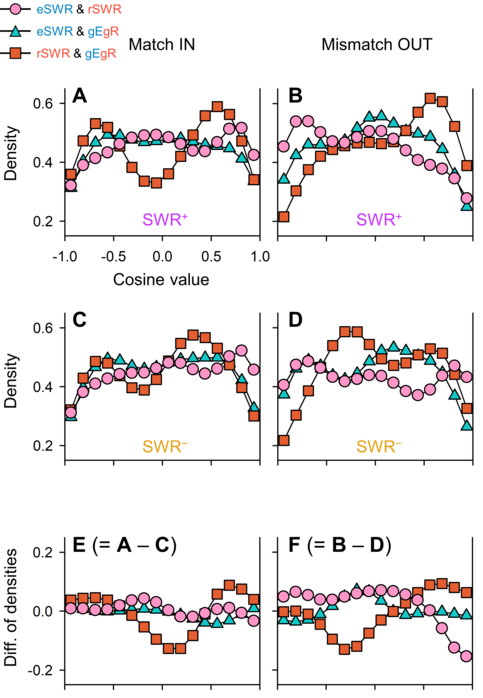
\includegraphics[width=0.5\textwidth]{./src/figures/.png/Figure_ID_07.png}
        	\caption{\textbf{
Directionality of Neural Trajectories in SWR based on Encoding and Retrieval States
}
\smallskip
\\
\textbf{\textit{A--B}} The Kernel Density Estimation (KDE) distribution of $\protect\overrightarrow{{\mathrm{eSWR^+}}} \cdot \protect\overrightarrow{{\mathrm{rSWR^+}}}$ (\textit{pink circles}), $\protect\overrightarrow{{\mathrm{eSWR^+}}} \cdot \protect\overrightarrow{{\mathrm{g_{E}g_{R}}}}$ (\textit{blue triangles}), and $\protect\overrightarrow{{\mathrm{rSWR^+}}} \cdot \protect\overrightarrow{{\mathrm{g_{E}g_{R}}}}$ (\textit{red rectangles}) in the Match IN (\textit{A}) and Mismatch OUT tasks (\textit{B}) are presented~\cite{li_functional_2023}. \textbf{\textit{C--D}} The corresponding distributions in these tasks are represented toggling $\mathrm{SWR^-}$ in place of $\mathrm{SWR^+}$~\cite{dimakopoulos_information_2022}. \textbf{\textit{E--F}} The differences between the distributions of $\mathrm{SWR^+}$ and $\mathrm{SWR^-}$ accentuate the SWR components (\textit{E} = \textit{C} $-$ \textit{A}; \textit{F} = \textit{B} $-$ \textit{D}), with the biphasic distributions of $\protect\overrightarrow{{\mathrm{rSWR^-}}} \cdot \protect\overrightarrow{{\mathrm{g_{E}g_{R}}}}$ emphasizing the neural fluctuations between encoding and retrieval states during the Sternberg task~\cite{borders_hippocampus_2022}. On the other hand, the Mismatch OUT task showed inverse directionality between $\protect\overrightarrow{{\mathrm{eSWR^+}}}$ and $\protect\overrightarrow{{\mathrm{rSWR^+}}}$ (\textit{pink circles}) which was not observed in the Match IN task (\textbf{\textit{E--F}})~\cite{naber_reciprocal_2001,van_strien_anatomy_2009}. Lastly, observed transitions from retrieval to encoding state for the SWR components occurred in both Match IN and Mismatch OUT tasks (\textit{red rectangles} in \textit{E--F})~\cite{niediek_reliable_2016,schomburg_spiking_2012}.
}
% width=0.5\textwidth
        	\label{fig:07}
        \end{figure*}
